\documentclass[9pt, xcolor=table]{beamer}

\usepackage[utf8]{inputenc}
\usepackage[round, comma]{natbib}
\usepackage{amsmath}
\usepackage{hyperref}
\usepackage{amsfonts}
\usepackage{verbatim}
\DeclareMathOperator*{\argmin}{arg\,min}



\mode<presentation> {

\usetheme{Madrid}

\setbeamertemplate{navigation symbols}{} 
\useinnertheme{circles}
\definecolor{greenish}{RGB}{0, 153, 76}
\usecolortheme[named=greenish]{structure}
}

\setbeamertemplate{headline}
{%
  \begin{beamercolorbox}[ht=3.5ex,dp=1.125ex,%
      leftskip=.3cm,rightskip=.3cm plus1fil]{section in head/foot}
    \usebeamerfont{section in head/foot}\usebeamercolor[fg]{section in head/foot}%
\insertsectionnavigationhorizontal{\paperwidth}{\hskip0pt plus1fill}{\hskip0pt plus1fill}
  \end{beamercolorbox}%
  \begin{beamercolorbox}[colsep=1.5pt]{middle separation line head}
  \end{beamercolorbox}
  \begin{beamercolorbox}[colsep=1.5pt]{lower separation line head}
  \end{beamercolorbox}
}

\title[Interpretation of black box models]{Interpretation of black box models using tree-based surrogate models \newline \small{Simulations}}
\author[Sofia Loibl]{Sofia Loibl}
\institute[LMU]{LMU München}
\date{\today}

\begin{document}

\begin{frame}
\titlepage 
\end{frame}


\begin{frame}
\frametitle{Outline} 
\tableofcontents 
\end{frame}


\section{Simulation basic Scenarios}
\begin{frame}{Simulation design}
Comparison of four MBT algorithms (SLIM, GUIDE, MOB, CTree)
with respect to performance, stability and interpretability.

\vspace{0.3cm}
\begin{itemize}
    \item 3 basic scenarios (linear smooth, linear abrupt, linear mixed)
    \item MBT as standalone (to measure accuracy of the MBT algorithms), surrogate for lm and surrogate for xgboost model (to measure fidelity)
    \item 3 different sample sizes (1000, 5000, 10000)
    \item 3 different pruning parameters (for alpha or impr)\end{itemize}
    
$\Rightarrow 3 \cdot 3 \cdot 3 \cdot 3 = 81$ Experiments for each MBT algorithm

\vspace{0.3cm}
100 Simulation runs

    
\end{frame}

\begin{frame}{Evaluation measures}
\begin{enumerate}
    \item Performance: $R^2$ and $MSE$ on training and test data
    \item Interpretability: number of leaf nodes
    \item Stability: Adjusted Rand Index (ARI)
\end{enumerate}
    
\end{frame}

\section{Linear Smooth}
\begin{frame}{Linear Smooth}
\textbf{Data}
\begin{itemize}
    \item $x_1,..., x_3 \sim U(-1,1)$ $\epsilon \sim N(0, sd_{data})$
    \item $ f_{ls}(x) = x_1 + 4   x_2 + 3   x_2   x_3 $
    \item $\epsilon \sim N(0, 0.1 sd(f_{ls}(x))$
    \item $y = f(x) + \epsilon$
\end{itemize}

\textbf{Settings:}
\begin{itemize}
    \item max tree depth = 7 
    \item min node size = 50    
\end{itemize}

\end{frame}

\begin{frame}{Linear Smooth}
\textbf{Comparison of MBTs as stand alone models}
\begin{table}
\caption{Mean simulation results on 100 simulation runs for \textbf{SLIM} as stand alone model on scenario Linear smooth with n = 1000 for different values of impr}
\centering 
\begin{tabular}[t]{r|r|r|r|r}
\hline
impr & number of leaf nodes & R2 train & R2 test & ARI\\
\hline
0.15 & 2.27 & 0.9587 & 0.9561 & 0.4734\\
\hline
0.10 & 10.08 & 0.9856 & 0.9831 & 0.2670\\
\hline
0.05 & 14.57 & 0.9908 & 0.9885 & 0.3259\\
\hline
\end{tabular}
\end{table}


\begin{table}

\caption{Mean simulation results on 100 simulation runs for \textbf{GUIDE} as stand alone model on scenario Linear smooth with n = 1000 for different values of impr}
\centering 
\begin{tabular}[t]{r|r|r|r|r}
\hline
impr & number of leaf nodes & R2 train & R2 test & ARI\\
\hline
0.15 & 2.25 & 0.9584 & 0.9560 & 0.5214\\
\hline
0.10 & 9.70 & 0.9856 & 0.9830 & 0.2940\\
\hline
0.05 & 14.49 & 0.9907 & 0.9884 & 0.3221\\
\hline
\end{tabular}
\end{table}
    
\end{frame}




\begin{frame}{Linear Smooth}
\begin{table}

\caption{Mean simulation results on 100 simulation runs for \textbf{MOB} as stand alone model on scenario Linear smooth with n = 1000 for different values of alpha}
\centering 
\begin{tabular}[t]{r|r|r|r|r}
\hline
alpha & number of leaf nodes & R2 train & R2 test & ARI\\
\hline
0.15 & 9.65 & 0.9899 & 0.9876 & 0.3473\\
\hline
0.10 & 10.96 & 0.9903 & 0.9879 & 0.3404\\
\hline
0.05 & 12.51 & 0.9906 & 0.9883 & 0.3691\\
\hline
\end{tabular}
\end{table} 


\begin{table}

\caption{Mean simulation results on 100 simulation runs for \textbf{CTree} as stand alone model on scenario Linear smooth with n = 1000 for different values of alpha}
\centering 
\begin{tabular}[t]{r|r|r|r|r}
\hline
alpha & number of leaf nodes & R2 train & R2 test & ARI\\
\hline
0.15 & 11.51 & 0.9901 & 0.9881 & 0.3764\\
\hline
0.10 & 12.89 & 0.9904 & 0.9884 & 0.3657\\
\hline
0.05 & 13.75 & 0.9905 & 0.9885 & 0.3633\\
\hline
\end{tabular}
\end{table}
\end{frame}



\begin{frame}{Linear Smooth}
For  $alpha= 0.001$ and $impr = 0.1$ the mean number of leaf nodes nodes is similar for the four MBT Algorithms, although it varies greatly for SLIM and CTree
\begin{figure}
    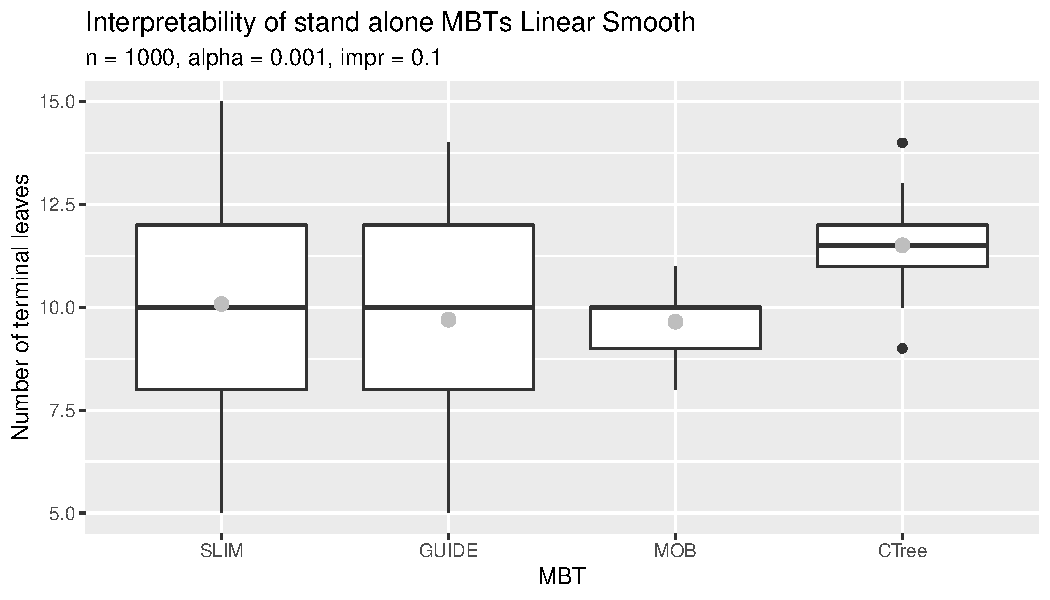
\includegraphics[width=11cm]{Figures/simulations/batchtools/basic_scenarios/linear_smooth/ls_1000_standalone_int.pdf}
\end{figure}   

    
\end{frame}

\begin{frame}{Linear Smooth}
\begin{figure}
    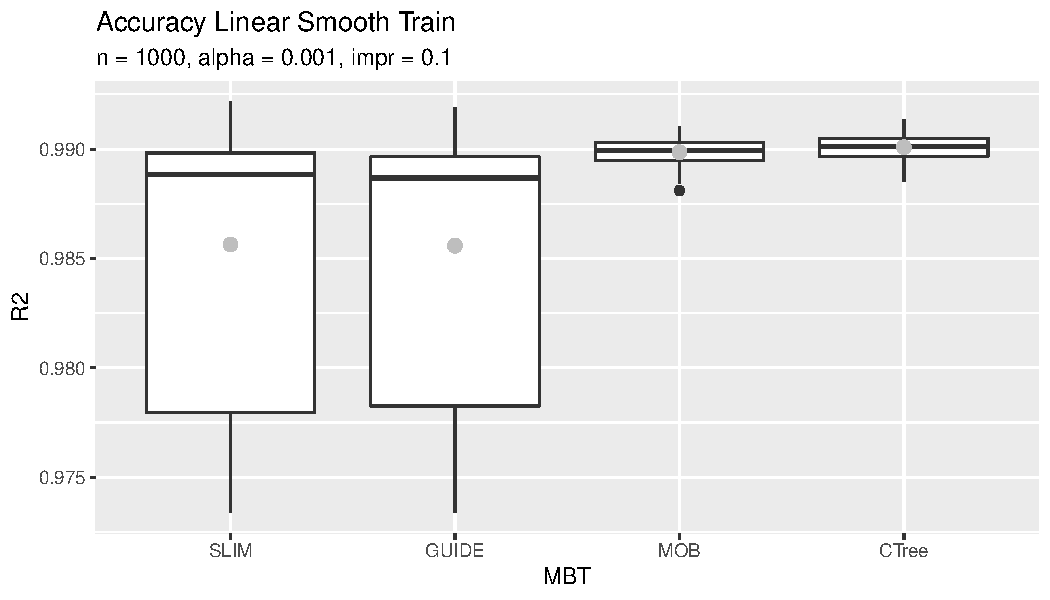
\includegraphics[width=11cm]{Figures/simulations/batchtools/basic_scenarios/linear_smooth/ls_1000_standalone_r2_train.pdf}
\end{figure}  
    
\end{frame}

\begin{frame}{Linear Smooth}
\begin{figure}
    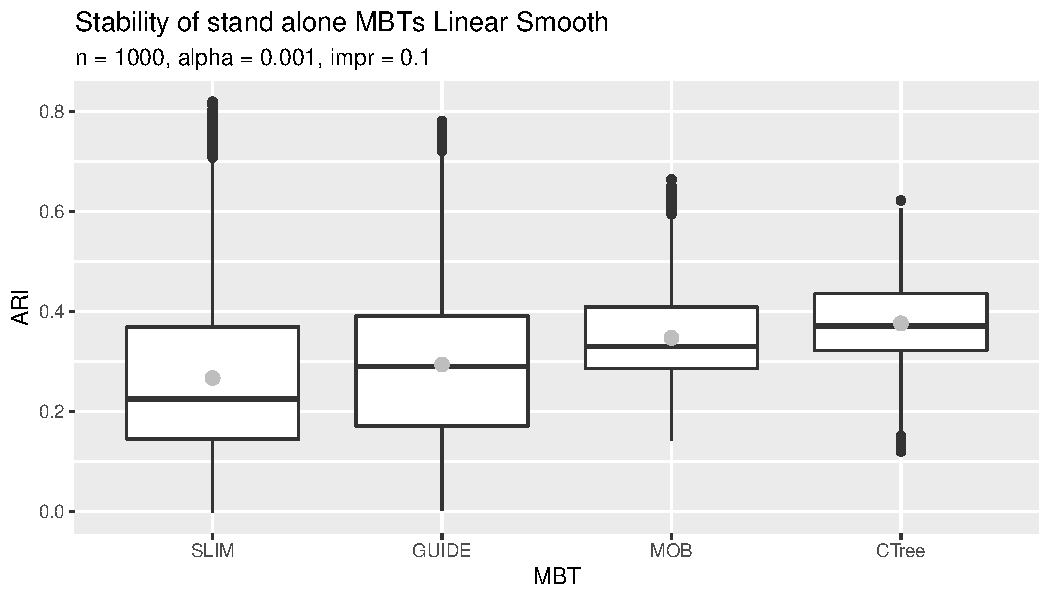
\includegraphics[width=11cm]{Figures/simulations/batchtools/basic_scenarios/linear_smooth/ls_1000_standalone_sta.pdf}
\end{figure}  
    
\end{frame}

\begin{frame}{Linear Smooth}
\textbf{Observations:}
\begin{itemize}
    \item All four algorithms achieve good performance
    \item The number of leaf nodes is high considering that the data generating process is very simple and involves only one interaction (increases even more with larger n)    
    \item SLIM and GUIDE are very sensitive regarding the choice of impr
    \item  If alpha and impr are chosen in this scenario so that the mean number of leaf nodes is similar, MOB and GUIDE provide more stable MBTs and have a better performance.

\end{itemize}

\textbf{Suggestion:}\\
Select a smaller maximum tree depth and a larger min node size in order to avoid large fluctuations and to obtain trees that are easier to interpret.

    
\end{frame}

\begin{frame}{Linear Smooth}
Comparison of MBTs used as surrogate models on lm predictions vs. used as stand alone models 
\begin{figure}
    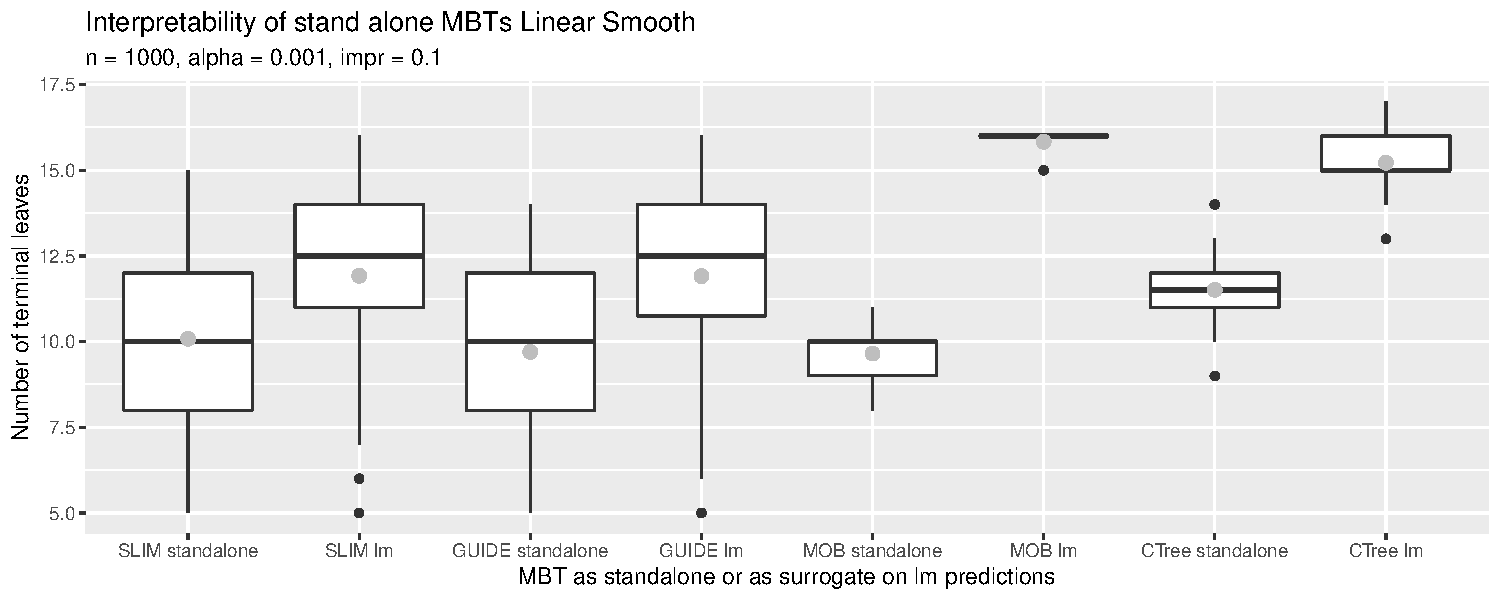
\includegraphics[width=11cm]{Figures/simulations/batchtools/basic_scenarios/linear_smooth/ls_1000_standalone_lm_int.pdf}
\end{figure}  
\end{frame}

\begin{frame}{Linear Smooth}
\begin{figure}
    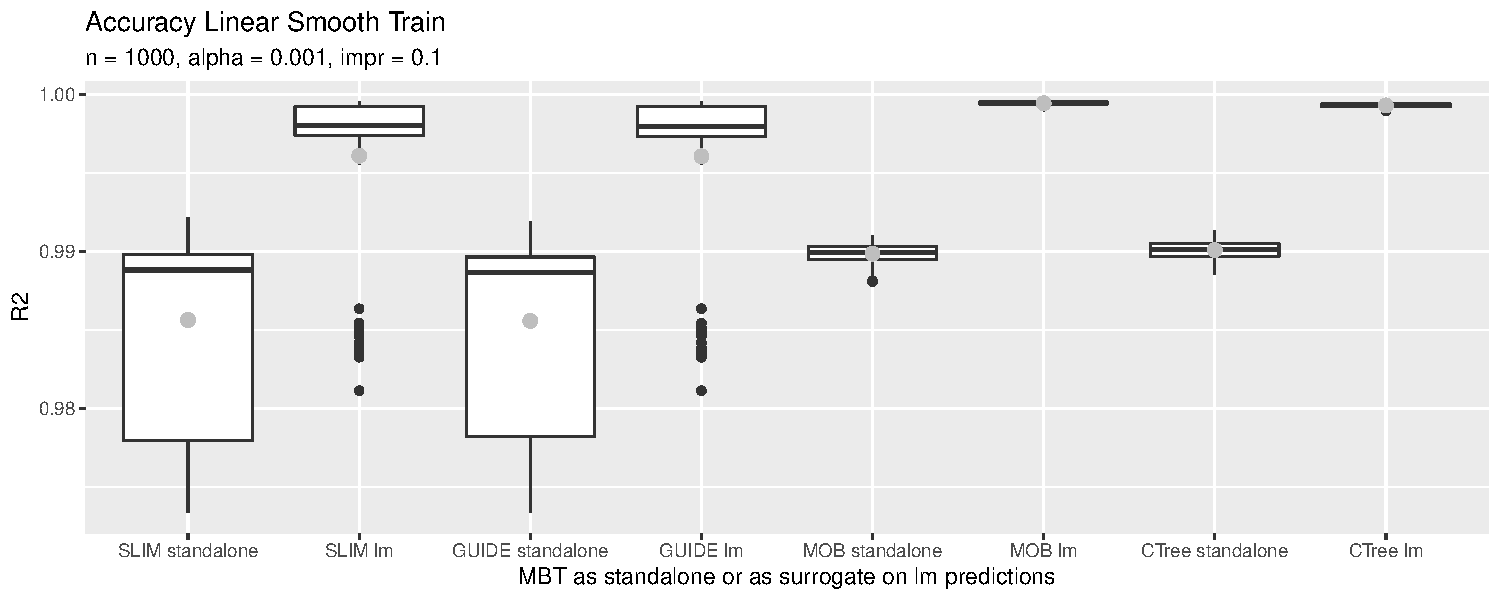
\includegraphics[width=11cm]{Figures/simulations/batchtools/basic_scenarios/linear_smooth/ls_1000_standalone_lm_r2_train.pdf}
\end{figure}  
\end{frame}


\begin{frame}{Linear Smooth}

\begin{figure}
    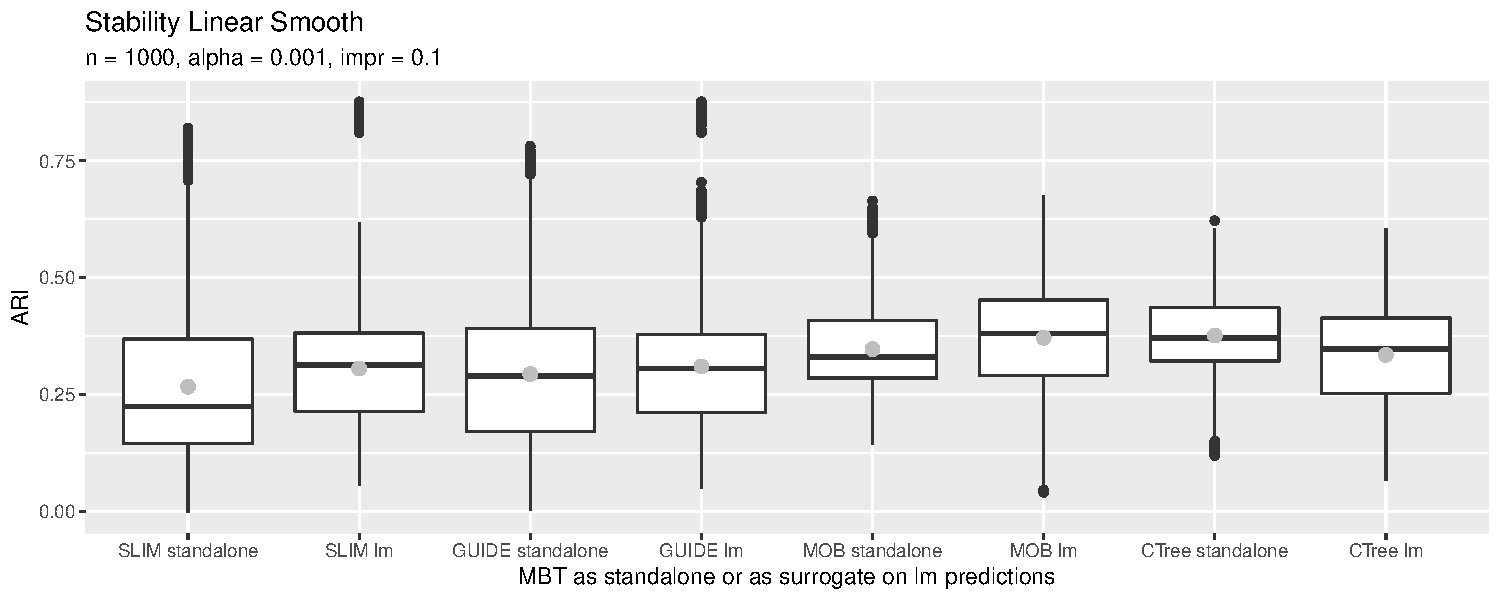
\includegraphics[width=11cm]{Figures/simulations/batchtools/basic_scenarios/linear_smooth/ls_1000_standalone_lm_sta.pdf}
\end{figure}  
\end{frame}

\begin{frame}{Linear Abrupt}
\begin{itemize}
    \item $x_1, x_2 \sim U(-1,1)$, $x_3 \sim Bern(0.5)$
    \item $ f_{la}(x) = x_{1} - 8  x_2 + 16  x_2  \mathbf{I}_{x_3 = 0} + 8  x_2  \mathbf{I}_{x_1 > mean(x_1)}$
    \item $\epsilon \sim N(0, 0.1 sd(f_{la}(x))$
    \item $y = f(x) + \epsilon$
\end{itemize}    
\end{frame}


\begin{frame}{Linear Abrupt}
\textbf{Comparison of MBTs as stand alone models}

\begin{table}
\caption{Mean simulation results on 100 simulation runs for \textbf{SLIM} and \textbf{GUIDE}  as stand alone model on scenario Linear abrupt with n = 1000 for different values of impr }
\centering
\begin{tabular}[t]{r|r|r|r|r}
\hline
impr & number of leaf nodes & R2 train & R2 test & ARI\\
\hline
0.15 & 2.01 & 0.8283 & 0.8255 & 0.9950\\
\hline
0.10 & 4.00 & 0.9889 & 0.9876 & 0.9742\\
\hline
0.05 & 4.00 & 0.9892 & 0.9878 & 0.9735\\
\hline
\end{tabular}
\end{table}    

Results of SLIM and GUIDE are identical in this special case
\end{frame}

\begin{frame}{Linear Abrupt}

\begin{table}

\caption{Mean simulation results on 100 simulation runs for \textbf{MOB} as stand alone model on scenario Linear abrupt with n = 1000 for different values of impr }
\centering
\begin{tabular}[t]{r|r|r|r|r}
\hline
alpha & number of leaf nodes & R2 train & R2 test & ARI\\
\hline
0.001 & 12.83 & 0.9660 & 0.9554 & 0.5520\\
\hline
0.010 & 14.24 & 0.9736 & 0.9640 & 0.5544\\
\hline
0.050 & 14.84 & 0.9751 & 0.9660 & 0.5555\\
\hline
\end{tabular}
\end{table}  

\begin{table}

\caption{Mean simulation results on 100 simulation runs for \textbf{CTree} as stand alone model on scenario Linear abrupt with n = 1000 for different values of impr }
\centering
\begin{tabular}[t]{r|r|r|r|r}
\hline
alpha & number of leaf nodes & R2 train & R2 test & ARI\\
\hline
0.001 & 11.96 & 0.9489 & 0.9384 & 0.6427\\
\hline
0.010 & 12.74 & 0.9501 & 0.9397 & 0.6316\\
\hline
0.050 & 13.59 & 0.9511 & 0.9409 & 0.6105\\
\hline
\end{tabular}
\end{table}
\end{frame}


\begin{frame}{Bibliography}
    \bibliography{bibliography}
    \bibliographystyle{dcu}

\end{frame}
\end{document}